\documentclass[prl,aps,epsf,showpacs,twocolumn,letterpaper]{revtex4}
\usepackage[T1]{fontenc}
\usepackage{newtxtext, newtxmath}
\usepackage{times}
\usepackage{graphicx}
\usepackage{tikz}
\usepackage{float}
\usepackage{latexsym,amsmath,amssymb,bm,euscript,braket}
\usepackage{color}
% \usepackage{subfigure}
% \usepackage{subcaption}
% \captionsetup{compatibility=false, justification=raggedright}
\usepackage{epstopdf}
\usepackage[colorlinks=true,linkcolor=blue,citecolor=blue]{hyperref}
\usepackage{hyperref}


% \renewcommand{\topmargin}{0.08in}
\newcommand{\oim}[1]{{\color{red}$\clubsuit$ #1}}

\bibliographystyle{apsrmp}



%%%%%%%%%%%%%%%%%%%%%%%%%%%%%%%%%%%%%%%%
% FOR MAC'S PERSONAL USE WITH "chktex" %
%%%%%%%%%%%%%%%%%%%%%%%%%%%%%%%%%%%%%%%%
% spaces after commands
% chktex-file 1
% spaces before '('
% chktex-file 36

%%%%%%%%%%%%%%%%%%%%%%%%%%%%%%%%%%%%
% Automatic numbering for sections %
%%%%%%%%%%%%%%%%%%%%%%%%%%%%%%%%%%%%
\let\oldsection\section
\renewcommand{\section}[1]{\stepcounter{section}\oldsection{\Roman{section}. #1}}

%%%%%%%%%%%%%%%%%%%%%%%%%%%%%
% Define the trace operator %
%%%%%%%%%%%%%%%%%%%%%%%%%%%%%
\DeclareMathOperator{\tr}{Tr}

%\newcommand{\oim}[1]{{\color{red}$\clubsuit$ #1}}

\bibliographystyle{apsrmp}

\begin{document}



\title{Many-Body Localization in  Spin Chain Systems with  Quasi-Periodic Fields}
\author{Mac Lee, Thomas R. Look, S. P. Lim and D. N. Sheng}

\affiliation{Department of Physics and Astronomy, California State University,
Northridge, California 91330, USA}


\begin{abstract} 
We study the many-body localization and transition in spin chain systems with  quasiperiodic  fields.
We identify the phase transition between the thermal and the many-body localized phases based on the finite-size
scaling of the entanglement entropy and the 
 fluctuations of the bipartite magnetization, which determines the  critical
strength of quasiperiodic fields to be around $W_{cl}\sim 1.7$ as the lower bound.  We further examine  the time evolution of the entanglement entropy of an initial product state,
where we find the entropy  shows  the power-law and logarithmic growth with time for the  thermal and MBL states, respectively.
The spin imbalance remains finite after  a long time, and  the spin glass ordering diverges with the system size in the MBL side.
 The quasiperiod fields  have been applied in different experimental systems, and our study
find such fields are  very efficient for driving  MBL phase.
\end{abstract}

\pacs{73.40.Hm, 71.30.+h, 73.20.Jc }
\maketitle


\section{Introduction}

The interplay of random disorder with many-body interactions has attracted a lot of recent research activity\cite{basko2006, oganesyan2007, pal2010, znidaric2008, huse2013, nandkishore2015, altman2015, huse2014, nandkishore2014, pekker_hilbert2014}.  The many-body localized (MBL) quantum state\cite{nandkishore2015, altman2015, huse2014, nandkishore2014, pekker_hilbert2014} of matter is distinctly different from both Anderson localized state  in non-interacting systems and the ergodic (thermal) state for interacting systems with weaker disorder.  The ergodic phase follows the  eigenstate thermalization hypothesis (ETH) which describes how an isolated self-interacting quantum system can thermalize under its own internal dynamics in agreement with quantum statistical mechanics\cite{deutsch1991, srednicki1994, rigol2008}.  A system in the MBL phase, on the other hand, fails to thermalize even for its highly excited eigenstates on any time scale, resulting in new statistics for such systems\cite{basko2006, oganesyan2007, pal2010, znidaric2008, huse2013, nandkishore2015, altman2015, huse2014, nandkishore2014, pekker_hilbert2014}.  Many remarkable properties of the MBL phase have been established\cite{nandkishore2015, altman2015, huse2013, nandkishore2014, oganesyan2007, pal2010, znidaric2008, rigol2008, serbyn2014, kwasigroch2014, yao2014, vasseur2015, huse2014, serbyn2013, ros2015, chandran2014, grover2014, agarwal2015, knap2015, luitz2015, devakul2015, torres2015, canovi2011, cuevas2012, bauer2013, kjall2014, luca2013, iyer2013, pekker_hilbert2014, johri2014, bardarson2012, andraschko2014, laumann2014, hickey2014, nanduri2014, barlev2014, imbrie2014, groverf2014, ponte2015, huang2015, you2015, serbyn2015, singh2015, barlev2015, deng2015, chen2015} based on extensive theoretical studies.  The existence of both the ergodic and MBL phases dictates  a novel dynamic quantum phase transition between them\cite{basko2006, pal2010, oganesyan2007, kjall2014, vosk_theory2014, potter2015trans, serbyn2015, agarwal2015, knap2015, lim2016, zhang2016, zhang2016a, yu2016, vedika2016, dumitrescu2017}.  Random disorder introduces rare Griffiths regions\cite{vosk_theory2014, potter2015trans, knap2015,luitz2015,lim2016} which may have singular contributions in driving such a phase transition, but there is still a limited quantitative understanding of their effects. Quasiperiodic fields break translational invariant and bring scattering between different spins in a controlled way.   Most numerical studies of the MBL transition have focused on models with random fields  for spin chains\cite{pal2010, kjall2014, luitz2015, yu2016, vedika2016}, while very interestingly  MBL phase and discrete time crystal have been identified in experimental systems with quasiperiodic fields\cite{serbyn2014,kwasigroch2014,yao2014,vasseur2015, bordia2015}.
Very recently,   the dynamic quantum phase transition has been analyzed with a close comparison between the quasiperiodic and random  fields, which point to the possibility of two universality classes for the quantum phase transition\cite{vedika2017, vedika2016}.

\begin{figure}
  \begin{tikzpicture}
    \node (o) at (0, 0) {};
    \node (a) [above] at (o) {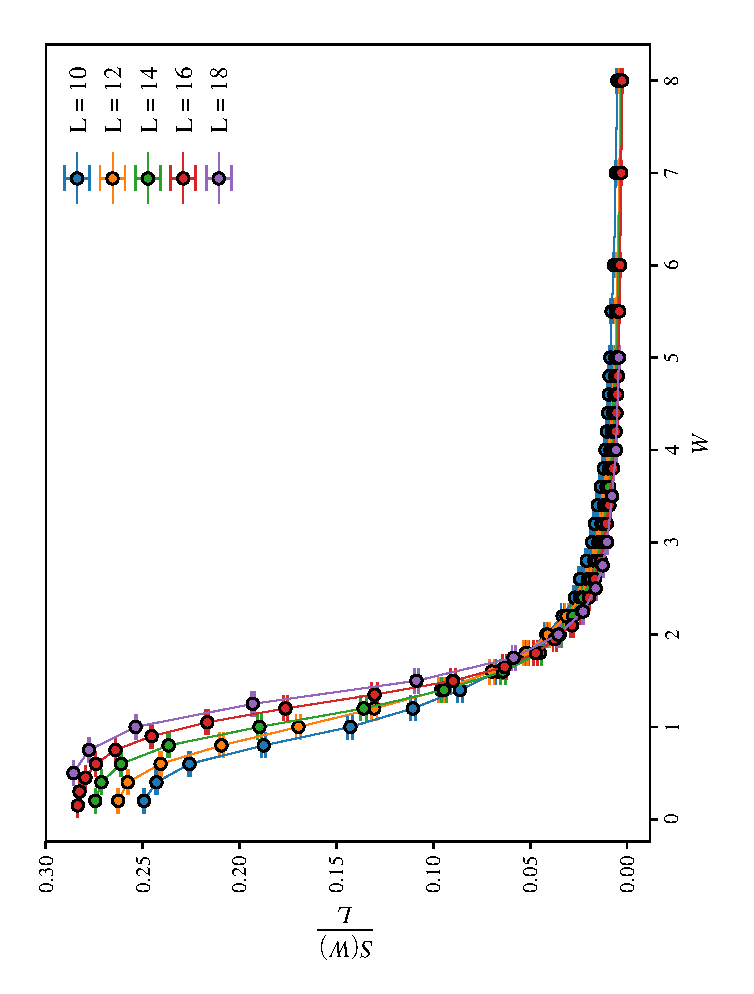
\includegraphics[angle=-90,width=0.85\linewidth]{entropy_plot.eps}};
    \node (b) [below] at (o) {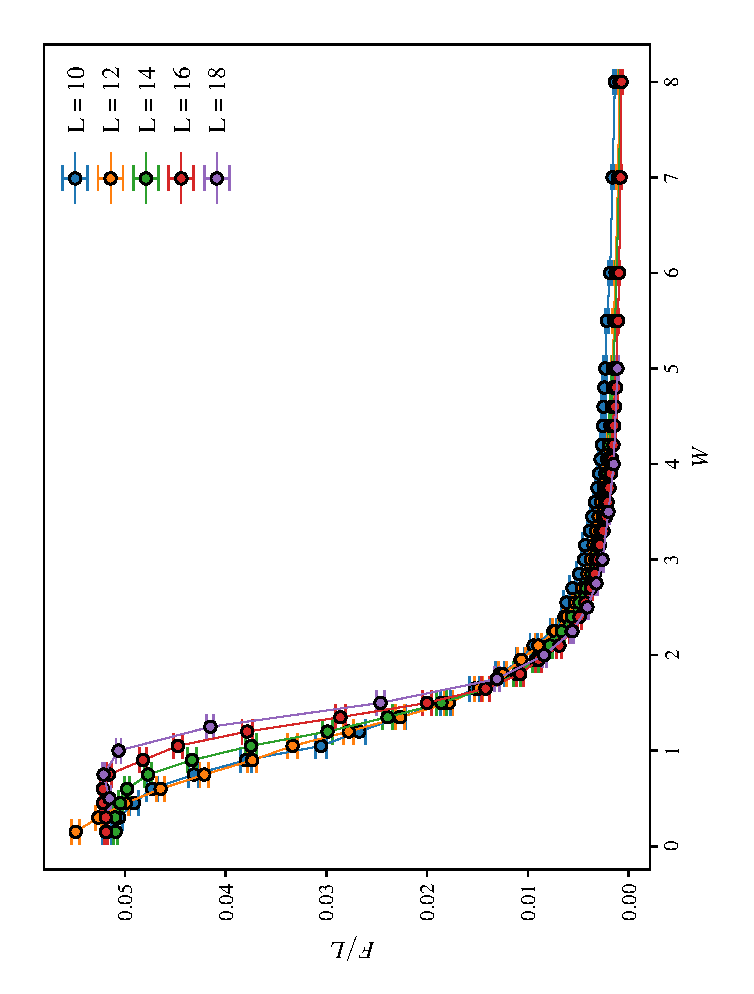
\includegraphics[angle=-90,width=0.85\linewidth]{variance_plot.eps}};
    \node [below, label=below:(a)] at (a.north west) {};
    \node [below, label=below:(b)] at (b.north west) {};
  \end{tikzpicture}
	\caption{
		(Color online) 
(a) The ratio of entanglement entropy over the number of system sites $S/L$ for $L=10-18$ at the energy density $\varepsilon=0$
 as a function of the  strength of the quasiperiodic fields $W$.  (b) 
The fluctuations of the half system magnetization over $L$ for $L=10-18$.
%For system sizes $L = 10-16$ we notice that both the bipartite entanglement entropy (top) and dispersion (bottom) decay with increasing $W$.  
Both graphs display crossing around $W_{cl}\sim1.7$, indicating a quantum phase transition at that point.  
%Agreement between these plots supports the conclusion that thermalization fails at high disorder strength.
}
	\label{fig1}
\end{figure}

\begin{figure}[b]
  \begin{tikzpicture}
    \node (o) at (0, 0) {};
    \node (a) [left] at (o)
    {\includegraphics[angle=-90,width=0.45\linewidth]{newfig1a.ps}};
    \node (b) [right] at (o)
    {\includegraphics[angle=-90,width=0.45\linewidth]{newfig1b.ps}};
    \node [below, label=below:(a)] at (a.north west) {};
    \node [below, label=below:(b)] at (b.north west) {};
  \end{tikzpicture}
	\caption{
		(Color online) (a) In this log-log plot, for systems with $W<W_c$ we observe power-law growth of entropy $S(t)$ which saturates at the $L=16$ Page value. (b) Semi-log plot of $S(t)$ with $W > W_c$ indicating logarithimc growth of $S(t)$.}
	\label{fig2}
\end{figure}


Time evolution of many-body systems have been studied for spin-chains with a randomly distributed fields\cite{kjall2014,luitz2016time}, which can be used to address the dynamics of the thermal to MBL phase transition\cite{nandkishore2015,vosk_theory2014,potter2015}.  After a global quantum quench, the power-law growth of bipartite entanglement entropy is observed for thermal states while logarithmic growth is found  for MBL states where  local memories of an initial product state persist for all time\cite{luitz2016time}.


In this paper we report on eigenstate and time-dependent studies of spin chains with quasiperiodic fields.  Through exact diagonalization (ED) and lanczos  Krylov space time evolution calculations, we find a dynamic quantum phase transition from the ergodic phase to the MBL phase that is similar to spin chains with random disordered fields.  However, systems with quasiperiodic fields  appear to be more efficient at localizing quantum states which is demonstrated by a smaller critical disorder, $W_{cl} \sim 1.7$ (as a lower bound) compared to similar estimate for systems with random  fields\cite{luitz2015} (where the critical disorder field strength
is around 3.5).  We also evolve randomly selected initial product states  and study how entanglement entropy and other observables behave as a function of time.  Similar to random field systems, we find that bipartite entanglement entropy in the thermal  and MBL phases experience power-law and logarithmic growth, respectively.  Interestingly, we also observe quasiperiodic oscillations of entanglement entropy on short timescales,  preservation of imbalance and spin glass order on  long timescale  characterizing  the MBL phase at larger quasiperiodic field side.  
The time evolution results suggest that the critical quasiperiodic field strength $W_c<3$,  which may be considered as an upper bound of the critical point.
Our results provide quantitative understanding of the MBL phase
for spin systems with quasiperiodic fields.   %% and  ushow that quasi-periodic systems are quantitatively similar to random disorder systems with respect to these standard statistical measurements.


\section{Theoretic model and  ergodic to many-body localized phase transition}


We study the Heisenberg spin-1/2 chain with  quasi-periodic fields
\begin{equation}
H = J\sum_{i=1}^{L-1} \mathbf{S}_i \cdot \mathbf{S}_{i+1} + W\sum_{i}^{L} \cos(2\pi c i+\phi) S_i^z \text{.}
\end{equation}
where $\mathbf{S}_i$ is the spin operator for site $i$, $J$ is the nearest neighbor coupling constant which we set to $J=1$, $W$ is the strength of the quasi-periodic fields, $c$ is an irrational wave number chosen to be $c=\sqrt{2}$, and $\phi$ is a random phase used to create different quasiperiodic field  configurations. $L$ is the number of sites (system length).  This model is similar to the one studied recently in \cite{vedika2017}, which also included second nearest neighboring transverse spin couplings.  In this paper, however, we focus on   the time-evolution of initial product states,  which has not been studied for systems with quasi-periodic fields.  We use open-boundary condition which allows for a larger window to observe the time evolution of physical quantities\cite{luitz2016time} before they saturate due to finite-size effects.  
%All results are obtained for highly excited states near the center of the eigenenergy spectrum.

\begin{figure*}[t]
	\centering
    (a) \includegraphics[angle=-90,width=.30\linewidth]{newfig1c.ps}
    (b) \includegraphics[angle=-90,width=.30\linewidth]{newfig1d.ps}
    (c) \includegraphics[angle=-90,width=.30\linewidth]{newfig1e.ps}
	\caption{
		(Color online) (a) For system sizes ranging from $12$ to $20$, at $W=1$, we observe that $S(t)$ increases rapidly
 until $t \sim 1$.  When $1<t<50$, $S(t)$ for all $L$ data fit into a straight line demonstrating robust power-law growth.  For larger $t$, we see that $S(t)$ saturates to $\frac{L}{2} \ln{2}$,  consistent with the thermal entropy of the ergodic phase. (b) At $W=2$, for smaller system sizes, we observe that $S(t)$ grows slower than predicted by the power-law; on the other hand, $L=20$ results behave as expected for a thermal state and the growth of its entropy over time follows the power-law. (c) At $W=3$, we notice that all $S(t)$ plots fit to a straight line in the semi-log plot, indicating logarithmic growth for the MBL state.}
	\label{fig3}
\end{figure*}


We perform Lanczos ED calculations to obtain energy eigenstates around the energy $E$ at a target energy density $\varepsilon$\cite{luitz2015}    for systems with different number of sites $L=10-18$ in the total $S_z=0$ sector.  Specifically, for each quasiperiodic field configuration, we first calculate the ground state energy $E_0$ and the maximum energy $E_\text{max}$, which are used to define the target energy density $\varepsilon = (E-E_0)/(E_\text{max} -E_0)$.
%Physical quantities\cite{luitz2015}  including the bipartite entanglement
%entropy,  energy level statistics and bipartite  fluctuation of the subsystem
%magnetization are obtained and averaged over disorder configurations and
%sometimes also averaged over  30 energy eigenstates with energies closest to
%the given energy density $\varepsilon$ as detailed below.
We first locate the critical point for the MBL phase transition based on the entanglement entropy and the fluctuations of the half-system magnetization\cite{luitz2015}.  The Von Neumann entanglement entropy of a system partitioned at  the middle with reduced density matrix $\rho_A$ is given by $S=- \tr (\rho_A \ln \rho_A)$.  We average the bipartite entanglement entropy over 30 ($L=12$) to 200 ($L=18$) eigenstates near target energy $E$ characterized by energy density $\varepsilon=0.5$ using the shift-invert method, and over $1000$ quasifield  configurations by choosing random $\phi$ between $(0, 2\pi)$.  As shown in Fig. 1(a), we plot the ratio of entanglement entropy over the number of system sites $S/L$ for different systems at energy density $\varepsilon=0.5$ from $L=10$ to $18$ as a function of quasi-periodic field strength $W$.  As $W\to0$ we see $S/L$ increases with $L$ which approaches the Page value ($S/L \sim 0.5\ln(2)$ for large $L$ limit) following the volume law of the ergodic phase.  For larger $W$, $S/L$ approaches zero indicating area law entanglement and non-ergodic behavior where the MBL state is realized.  With varying $W$, all data points approximately cross each other around a critical value $W_{cl} \sim 1.7$.  We compare the entanglement entropy behavior with the bipartite fluctuations $F$ of the subsystem magnetization $S^z_A$~\cite{luitz2015,song2012}, which is defined as $F=\braket{{S^{z}_A}^2} - \braket{S^z_A}^2$ as shown in Fig. 1(b).  We see that $F/L$ increases on the small $W$ side, while it becomes vanishing small on the larger $W$ side.  The $F/L$ curves for different $L$ approximately cross each other around the  critical field strength $W_{cl}\sim1.7$, consistent with the behavior of the entanglement entropy.  In fact, we see that there is an approximately proportional relationship between $S$ and $F$  for all $W$ region. 
We also note that,  the crossing points between larger $L$ curves move towards the larger $W$ side.  This feature was also observed in a different models for quasi-periodic systems as well as for random disorder systems\cite{vedika2016, vedika2017}.  This feature indicates the $W_{cl}$ we observed is a lower bound for the critical point of the  dynamic quantum phase transition.  


We now analyze the finite-size  scaling properties of the MBL transition for  the quasiperiodic field model.
Crossing  the quantum phase transition,  we expect that the  entanglement entropy over the system length  $S/L$ and the fluctuations of the
half system magnetization over the system length  $F/L$   should  be a function of
$L/\xi\sim  L|W-W_c|^{\nu}$, where the correlation length $\xi$ diverges   at the transition point in a power-law way with an  exponent $\nu$.
As shown in Fig. 2(a-b),  we find that these quantities for all system lengthes can indeed be collapsed into one curve
in a form $f(L^{1/\nu}|W-W_c|)$ by using  the proper critical $W_c\sim 1.7$ and the scaling exponent $\nu\sim 1$, which give the best collapsing effect.
The obtained exponent $\nu$ is in good agreement with the results of 
 Khemani  et al.\cite{vedika2017}



%We then use the level statistics analysis from random matrix theory\cite{atas2013,oganesyan2007} to probe the localization-delocalization characteristics of the energy eigenstates.  
%In the delocalized  regime, the level-spacing  distribution is described by the
%Gaussian orthogonal ensemble (GOE) statistics, which represents extended levels
%with level-repulsion  between them because of the overlap of  energy
%eigenstates in real space.  In the localized regime, the level-spacing
%distribution  is determined by Poisson statistics as  wave-functions close in
%energy are exponentially localized with no level repulsion between
%them\cite{mehta1991}.
%In energy spectrum analysis\cite{luitz2015}, we define the adjacent energy gap $\delta_n=E_n-E_{n-1}$ as the energy difference between the $n$-th and $(n-1)$-th eigenstates, then the adjacent gap ratio can be defined as $r_n=\min(\delta_n, \delta_{n+1})/\max(\delta_n, \delta_{n+1})$.  We average the gap ratio $r=\langle r_n\rangle$ over $30-200$ states near the spectrum center at $\varepsilon=0.5$ and more than 1000 random potential configurations for each given disorder strength $W$.  As shown in Fig. 1(c), we see that at the small $W$ side, $r$ approaches the Gaussian orthogonal ensemble value ($0.5307$), which represents extended levels with level-repulsion between them because of the overlap of energy eigenstates in real space.  On the stronger $W$ side, $r$ reaches the Poisson value $(2\ln2-1\simeq 0.3863)$ for larger systems representing the level statistics of localized states, where states close in energies are exponentially localized with exponential small overlap without level repulsion between them\cite{mehta1991}.  A similar level crossing for all curves is also seen in Fig.1(c), indicating the same critical point for the dynamic quantum phase transition.  


\subsection{Time-evolution of quantum state}


We study the non-equilibrium quantum dynamics of the quasiperiodic systems after a global quantum quench.  Here we start from selecting a product state $\ket{\Psi(0)}=\ket{\sigma_1, \sigma_2, \ldots , \sigma_L}$  
with an avarage energy close to the target energy determined by the energy density $\varepsilon=0$ at the time $t=0$ after the quench, where $\sigma_i=\pm$ represents the spin-z component $\pm 1/2$ (with setting $\hbar=1$)
at site $i$.  The state at time $t$ can be obtained as $\ket{\Psi(t)} = e^{-iHt}\ket{\psi(0)}=e^{-iH\Delta t}\ket{\psi(t-\Delta t)}$. 
  We calculate the time evolution of an initial  state  $|\Psi_0>$ based on  a projection of the Hamiltonian to the Krylov space spanned by $\ket{\Psi_0}$, $H\ket{\Psi_0}$, \ldots, $H^n\ket{\Psi_0}$.
We calculate all eigenstates in this space to obtain the time-evolution operator\cite{luitz2015}.  Using a reasonably small time step $\delta t \sim 0.2/J$ allows for highly accurate results with a small $n=30-60$.  All time-evolution results are being averaged
over more than 1000 quasiperiodic field configurations. 

We first discuss the general behavior of the entanglement entropy as a function of time.  On the small $W$ side shown in Fig. 2(a), we find that the entropy $S(t)$ exhibits power-law growth in time $t$ before it reaches the saturated value $\frac L 2 \ln2$ at long time limit in agreement with the ETH of the thermal phase.  On the larger $W$ side, we find a much slower growth, which can be fit with a logarithmic growth function as shown in Fig. 2(b) for $W=3-5$.  
We now analyze the finite-size scaling behavior of $S(t)$ for $L=12-20$.  For small $W=1$ as shown in Fig. 3(a), we find that the initial growth ($t\sim 1$) of $S(t)$ is exponential and system size independent.  For the intermediate time regime, $S(t)$ experiences power-law growth as domenstrated by the linear behavior in the logarithmic plots until the finite-size effect sets in.  With the increase of $L$, we find a wider time interval for the power-law growth of $S(t)$.  Interestingly, we see very similar behavior and a smaller window for power-law growth of $S(t)$ for $W=2$.  The power-law growth indicated by the straight line in the Fig.3(b) is most clear for larger system size $L=20$.  This is a strong indication that the $W=2$  is in the thermal phase consistent with the moving of the crossing point toward larger $W$ with the increase of $L$ observed in Fig. 1.  We then look into $S(t)$ at $W=3$ where we observe that for small $t$, $S(t)$ grows rapidly  while the initial product state evolves to a superposition state for $t\sim 1$, which is then followed by some oscillations of $S(t)$.  With further increase of $t$, we find a logarithmic growth of $S(t)$ for a time range of more than two orders of magnitude.  The range of $t$ for logarithmic growth of $S(t)$ becomes larger with the increase of $W$.  These results confirm an MBL phase with similar behavior to the random field case studied by Luitz et. al\cite{luitz2015}.  

Now we turn to  spin correlations during the time evolution.  We start from the product state $|\Psi(0)>$ where the $\sigma_z$ on each site is $\pm 1/2$ while the total $S_z$ of all sites are zero.  We define the following time correlator for $\sigma_z$ as 
\begin{equation}
I(t)=\frac{4}{L} \sum_{j=1}^L \braket{\Psi(0)|S_j^z(0)S_j^z(t)|\Psi(0)} \text{,} \label{eq:imb}
\end{equation}
which detects the total imbalance of $\sigma_z$.  As shown in Fig.4(a), we find a systematic change of the properties of $I(t)$ as $W$ is varied.  For smaller $W=0.5$ and $1$, we see that the long time behavior of imbalance $I(t)$ is dominated by  power-law decay $t^{-\zeta}$, and at the large $t$ limit $\sigma_z$ on a site becomes uncorrelated with the initial condition and $I(t)$ approaches zero.  For intermediate $W=1.5$ and $2$, a similar power-law behavior is obtained with a much smaller decay power $\zeta$, indicating the longer time scale required to approach equilibrium spin correlations for these thermal states near the transition point to the MBL phase.  On the MBL side with $W=3$ and $4$, we see that the $I(t)$ is near constant at large $t$ limit with a near vanishing decay exponent ($\zeta \sim 0$).
IN Fig. 4(b),  we show the decay exponent $\zeta$ as a function of $W$,  where we find that the critical point for the transition to MBL phase is close to $W_c \sim 2.5\pm 0.04$ in consistent
with the conjecture that $W_{cl}\sim 1.7$ is only the lower bound of the critical point, though for given range of system sizes $L=10-18$
 it does give the best collapsing of the finite sizes entropy and fluctuation data as (for highly excited eigenstates) as show in Fig. 2.

%	\includegraphics[angle=-90,width=.95\linewidth]{newfig2a.ps}\\
\begin{figure}[h]
        \centering
	\includegraphics[width=0.49\linewidth]{imbalance_fit.ps} \includegraphics[width=0.49\linewidth]{zeta_plot.ps}

	\includegraphics[angle=-90,width=.95\linewidth]{newfig2b.ps}\\
	\caption{
		(Color online) (a) Imbalance $I(t)$ for a $L=16$ system with $W=0.5-6$.  At small values of $W$, we notice the $I(t)$ of the system decays rapidly; however, when $W$ is increased beyond $W>2$, $I(t)$  ceases decaying and remains at a certain level.  This is consistent with the MBL behavior where the initial values of the local observables for each site $i$ is preserved. (b) Fitting parameter $\zeta$ for the power-law decay exponent as a function of $W$. (c) Spin glass order as defined in eq.\ref{eq:sgo}. At small values of $W$, correlations between spins are short ranged and $\chi(t)$ decays to $1$ over time; at large values of $W$, $\chi(t)$ remains close to its initial value even at very long time, further corroborating our assertion of a quantum phase transition.}
	\label{fig4}
\end{figure}

For comparison, we also study spin glass order for the MBL phase.  The spin-flip from the Heisenberg term will create domain walls.  If the domain walls are confined together, a spin-glass order can develop.  We define the spin glass order parameter 
\begin{equation}
\chi^{SG}=\frac 1 L \sum_{i,j=1}^L \braket{\Psi(t)|S_i^zS_j^z|\Psi(t)}^2 \text{,} \label{eq:sgo}
\end{equation}
which can diverge with $L$ in the spin-glass ordered phase.  As shown in Fig.4(c), we see behavior very similar  to $I(t)$.  For smaller $W=1-2$, we see that $\chi(t)$ decreases with $t$ in power-law fashion, while it maintains a large value in the long time limit for larger $W>2$.  Our results indicate a jump of the spin glass order at the thermal to MBL transition.  In Fig.5, we see that both $I(t)$ and $\chi(t)/L$ show very weak size dependence at $W=3$ and remain long zero at long time and large system size limits, which fully establishes the robustness of the MBL phase.  

\begin{figure}[h]
	\centering
	\includegraphics[angle=-90,width=0.95\linewidth]{newfig3a.ps}\\ \includegraphics[angle=-90,width=0.92\linewidth]{newfig3b.ps}\\
	\caption{
		(Color online) 
		 (a) Imbalance $I(t)$ for a $L=12-20$ systems at $W=3$. $I(t)$ is insensitive to system size $L$.  It 
shows initial oscillation at shorter times, and it stays at nonzero
value at the long time limit.   (b) Spin glass order $\chi^{SG}(t)/L$ saturates to finite nonzero value indicating the divergent 
behavior with $L$. }
	\label{fig4}
\end{figure}


%\begin{figure}[h]
%	\centering
%	\includegraphics[width=\linewidth]{fit_tail.ps}
%	\caption{(Color online) (a) \bf Needs to be written}
%	\label{fig7}
%\end{figure}

\subsection{Summary and Discussions}

We have studied the many-body localization and quantum phase transition in spin chain systems with the presence of the quasiperiodic fields.    
Based on the entanglement entropy and the flutuation of the half system magnetization studies, 
we find the lower bound of critical field strength $W_{cl}\sim 1.7$ for 
the dynamic quantum phase  transition from the thermal phase 
to the MBL phase  driven by the quasiperiodic fields. Interestingly,   for $W$ just above $W_{cl}$, we identify the
entanglement entropy after a global quench following a power-law growth with time in consistent with the behavior of the
thermal phase.   From the scaling behavior of the spin imbalance and spin glass ordering, 
we identify the divergent spin glass ordering for $W\geq 3$.    Overall, the finite size effect in such a quasiperiodic system turns
out to be less important as the scaling behavior in the intermediate regime near the transition appears to be clear following either
thermal behavior ($W \sim 2 $) or MBL characteristics ($W\sim 3$), which provide a best estimate of the transition point to be $W_c=2.5\pm 0.4$.  
Our results provide quantitative understanding of the effect of the quasiperiodic fields,  which are more efficient in driving
MBL physics than the random  fields due to importance of the the rare   Griffiths regions in the random
fields models.
It would be very interesting to further identify the phase diagram for quantum states at different energy density and reexamine
the possibility of  the existence of the mobility edge  in such systems.  Another interesting direction is to explore
the MBL phase transition in ladder systems with coupled spin chains, which provides information about the MBL physics
in two dimension.   


                                 

{\bf Acknowledgments} --- The first two authors contributed equally to this
work.  This work is supported by US National Science Foundation  Grants PREM
DMR-1205734 (ML, TRL) and DMR-1408560 (SPL, DNS).


%%%%%%%%%%%%%%%%%%%%%%%%%%%%%%%%%%%% References
%\bibliographystyle{apsrev}
%\bibliography{quasi_mbl}


\begin{thebibliography}{62}
\expandafter\ifx\csname natexlab\endcsname\relax\def\natexlab#1{#1}\fi
\expandafter\ifx\csname bibnamefont\endcsname\relax
  \def\bibnamefont#1{#1}\fi
\expandafter\ifx\csname bibfnamefont\endcsname\relax
  \def\bibfnamefont#1{#1}\fi
\expandafter\ifx\csname citenamefont\endcsname\relax
  \def\citenamefont#1{#1}\fi
\expandafter\ifx\csname url\endcsname\relax
  \def\url#1{\texttt{#1}}\fi
\expandafter\ifx\csname urlprefix\endcsname\relax\def\urlprefix{URL }\fi
\providecommand{\bibinfo}[2]{#2}
\providecommand{\eprint}[2][]{\url{#2}}

\bibitem[{\citenamefont{{Altman} and {Vosk}}(2015)}]{altman2015}
\bibinfo{author}{\bibfnamefont{E.}~\bibnamefont{{Altman}}} \bibnamefont{and}
  \bibinfo{author}{\bibfnamefont{R.}~\bibnamefont{{Vosk}}},
  \bibinfo{journal}{Annu. Rev. Cond. Matt. Phys.} \textbf{\bibinfo{volume}{6}},
  \bibinfo{pages}{383} (\bibinfo{year}{2015}).

\bibitem[{\citenamefont{{Huse} et~al.}(2014)\citenamefont{{Huse},
  {Nandkishore}, and {Oganesyan}}}]{huse2014}
\bibinfo{author}{\bibfnamefont{D.~A.} \bibnamefont{{Huse}}},
  \bibinfo{author}{\bibfnamefont{R.}~\bibnamefont{{Nandkishore}}},
  \bibnamefont{and}
  \bibinfo{author}{\bibfnamefont{V.}~\bibnamefont{{Oganesyan}}},
  \bibinfo{journal}{\prb} \textbf{\bibinfo{volume}{90}}, \bibinfo{eid}{174202}
  (\bibinfo{year}{2014}).

\bibitem[{\citenamefont{{Nandkishore} et~al.}(2014)\citenamefont{{Nandkishore},
  {Gopalakrishnan}, and {Huse}}}]{nandkishore2014}
\bibinfo{author}{\bibfnamefont{R.}~\bibnamefont{{Nandkishore}}},
  \bibinfo{author}{\bibfnamefont{S.}~\bibnamefont{{Gopalakrishnan}}},
  \bibnamefont{and} \bibinfo{author}{\bibfnamefont{D.~A.}
  \bibnamefont{{Huse}}}, \bibinfo{journal}{\prb} \textbf{\bibinfo{volume}{90}},
  \bibinfo{eid}{064203} (\bibinfo{year}{2014}).

\bibitem[{\citenamefont{{Nandkishore} and {Huse}}(2015)}]{nandkishore2015}
\bibinfo{author}{\bibfnamefont{R.}~\bibnamefont{{Nandkishore}}}
  \bibnamefont{and} \bibinfo{author}{\bibfnamefont{D.~A.}
  \bibnamefont{{Huse}}}, \bibinfo{journal}{Annu. Rev. Cond. Matt. Phys.}
  \textbf{\bibinfo{volume}{6}}, \bibinfo{pages}{15} (\bibinfo{year}{2015}).

\bibitem[{\citenamefont{{Oganesyan} and {Huse}}(2007)}]{oganesyan2007}
\bibinfo{author}{\bibfnamefont{V.}~\bibnamefont{{Oganesyan}}} \bibnamefont{and}
  \bibinfo{author}{\bibfnamefont{D.~A.} \bibnamefont{{Huse}}},
  \bibinfo{journal}{\prb} \textbf{\bibinfo{volume}{75}}, \bibinfo{eid}{155111}
  (\bibinfo{year}{2007}).

\bibitem[{\citenamefont{{Pal} and {Huse}}(2010)}]{pal2010}
\bibinfo{author}{\bibfnamefont{A.}~\bibnamefont{{Pal}}} \bibnamefont{and}
  \bibinfo{author}{\bibfnamefont{D.~A.} \bibnamefont{{Huse}}},
  \bibinfo{journal}{\prb} \textbf{\bibinfo{volume}{82}}, \bibinfo{eid}{174411}
  (\bibinfo{year}{2010}).

\bibitem[{\citenamefont{{{\v Z}nidari{\v c}} et~al.}(2008)\citenamefont{{{\v
  Z}nidari{\v c}}, {Prosen}, and {Prelov{\v s}ek}}}]{znidaric2008}
\bibinfo{author}{\bibfnamefont{M.}~\bibnamefont{{{\v Z}nidari{\v c}}}},
  \bibinfo{author}{\bibfnamefont{T.}~\bibnamefont{{Prosen}}}, \bibnamefont{and}
  \bibinfo{author}{\bibfnamefont{P.}~\bibnamefont{{Prelov{\v s}ek}}},
  \bibinfo{journal}{\prb} \textbf{\bibinfo{volume}{77}}, \bibinfo{eid}{064426}
  (\bibinfo{year}{2008}).

\bibitem[{\citenamefont{{Basko} et~al.}(2006)\citenamefont{{Basko}, {Aleiner},
  and {Altshuler}}}]{basko2006}
\bibinfo{author}{\bibfnamefont{D.~M.} \bibnamefont{{Basko}}},
  \bibinfo{author}{\bibfnamefont{I.~L.} \bibnamefont{{Aleiner}}},
  \bibnamefont{and} \bibinfo{author}{\bibfnamefont{B.~L.}
  \bibnamefont{{Altshuler}}}, \bibinfo{journal}{Annals of Physics}
  \textbf{\bibinfo{volume}{321}}, \bibinfo{pages}{1126} (\bibinfo{year}{2006}).

\bibitem[{\citenamefont{{Pekker} et~al.}(2014)\citenamefont{{Pekker}, {Refael},
  {Altman}, {Demler}, and {Oganesyan}}}]{pekker_hilbert2014}
\bibinfo{author}{\bibfnamefont{D.}~\bibnamefont{{Pekker}}},
  \bibinfo{author}{\bibfnamefont{G.}~\bibnamefont{{Refael}}},
  \bibinfo{author}{\bibfnamefont{E.}~\bibnamefont{{Altman}}},
  \bibinfo{author}{\bibfnamefont{E.}~\bibnamefont{{Demler}}}, \bibnamefont{and}
  \bibinfo{author}{\bibfnamefont{V.}~\bibnamefont{{Oganesyan}}},
  \bibinfo{journal}{Phys. Rev. X} \textbf{\bibinfo{volume}{4}},
  \bibinfo{eid}{011052} (\bibinfo{year}{2014}).

\bibitem[{\citenamefont{{Huse} et~al.}(2013)\citenamefont{{Huse},
  {Nandkishore}, {Oganesyan}, {Pal}, and {Sondhi}}}]{huse2013}
\bibinfo{author}{\bibfnamefont{D.~A.} \bibnamefont{{Huse}}},
  \bibinfo{author}{\bibfnamefont{R.}~\bibnamefont{{Nandkishore}}},
  \bibinfo{author}{\bibfnamefont{V.}~\bibnamefont{{Oganesyan}}},
  \bibinfo{author}{\bibfnamefont{A.}~\bibnamefont{{Pal}}}, \bibnamefont{and}
  \bibinfo{author}{\bibfnamefont{S.~L.} \bibnamefont{{Sondhi}}},
  \bibinfo{journal}{\prb} \textbf{\bibinfo{volume}{88}}, \bibinfo{eid}{014206}
  (\bibinfo{year}{2013}).

\bibitem[{\citenamefont{{Rigol} et~al.}(2008)\citenamefont{{Rigol}, {Dunjko},
  and {Olshanii}}}]{rigol2008}
\bibinfo{author}{\bibfnamefont{M.}~\bibnamefont{{Rigol}}},
  \bibinfo{author}{\bibfnamefont{V.}~\bibnamefont{{Dunjko}}}, \bibnamefont{and}
  \bibinfo{author}{\bibfnamefont{M.}~\bibnamefont{{Olshanii}}},
  \bibinfo{journal}{\nat} \textbf{\bibinfo{volume}{452}}, \bibinfo{pages}{854}
  (\bibinfo{year}{2008}).

\bibitem[{\citenamefont{{Deutsch}}(1991)}]{deutsch1991}
\bibinfo{author}{\bibfnamefont{J.~M.} \bibnamefont{{Deutsch}}},
  \bibinfo{journal}{\pra} \textbf{\bibinfo{volume}{43}}, \bibinfo{pages}{2046}
  (\bibinfo{year}{1991}).

\bibitem[{\citenamefont{{Srednicki}}(1994)}]{srednicki1994}
\bibinfo{author}{\bibfnamefont{M.}~\bibnamefont{{Srednicki}}},
  \bibinfo{journal}{\pre} \textbf{\bibinfo{volume}{50}}, \bibinfo{pages}{888}
  (\bibinfo{year}{1994}).

\bibitem[{\citenamefont{{Agarwal} et~al.}(2015)\citenamefont{{Agarwal},
  {Gopalakrishnan}, {Knap}, {M{\"u}ller}, and {Demler}}}]{agarwal2015}
\bibinfo{author}{\bibfnamefont{K.}~\bibnamefont{{Agarwal}}},
  \bibinfo{author}{\bibfnamefont{S.}~\bibnamefont{{Gopalakrishnan}}},
  \bibinfo{author}{\bibfnamefont{M.}~\bibnamefont{{Knap}}},
  \bibinfo{author}{\bibfnamefont{M.}~\bibnamefont{{M{\"u}ller}}},
  \bibnamefont{and} \bibinfo{author}{\bibfnamefont{E.}~\bibnamefont{{Demler}}},
  \bibinfo{journal}{Physical Review Letters} \textbf{\bibinfo{volume}{114}},
  \bibinfo{eid}{160401} (\bibinfo{year}{2015}), \eprint{1408.3413}.

\bibitem[{\citenamefont{{Andraschko} et~al.}(2014)\citenamefont{{Andraschko},
  {Enss}, and {Sirker}}}]{andraschko2014}
\bibinfo{author}{\bibfnamefont{F.}~\bibnamefont{{Andraschko}}},
  \bibinfo{author}{\bibfnamefont{T.}~\bibnamefont{{Enss}}}, \bibnamefont{and}
  \bibinfo{author}{\bibfnamefont{J.}~\bibnamefont{{Sirker}}},
  \bibinfo{journal}{Phys. Rev. Lett.} \textbf{\bibinfo{volume}{113}},
  \bibinfo{eid}{217201} (\bibinfo{year}{2014}).

\bibitem[{\citenamefont{{Bar Lev} and {Reichman}}(2014)}]{barlev2014}
\bibinfo{author}{\bibfnamefont{Y.}~\bibnamefont{{Bar Lev}}} \bibnamefont{and}
  \bibinfo{author}{\bibfnamefont{D.~R.} \bibnamefont{{Reichman}}},
  \bibinfo{journal}{\prb} \textbf{\bibinfo{volume}{89}}, \bibinfo{eid}{220201}
  (\bibinfo{year}{2014}).

\bibitem[{\citenamefont{{Bar Lev} and {Reichman}}(2015)}]{barlev2015}
\bibinfo{author}{\bibfnamefont{Y.}~\bibnamefont{{Bar Lev}}} \bibnamefont{and}
  \bibinfo{author}{\bibfnamefont{D.~R.} \bibnamefont{{Reichman}}},
  \bibinfo{journal}{ArXiv e-prints}  (\bibinfo{year}{2015}),
  \eprint{1508.05391}.

\bibitem[{\citenamefont{{Bardarson} et~al.}(2012)\citenamefont{{Bardarson},
  {Pollmann}, and {Moore}}}]{bardarson2012}
\bibinfo{author}{\bibfnamefont{J.~H.} \bibnamefont{{Bardarson}}},
  \bibinfo{author}{\bibfnamefont{F.}~\bibnamefont{{Pollmann}}},
  \bibnamefont{and} \bibinfo{author}{\bibfnamefont{J.~E.}
  \bibnamefont{{Moore}}}, \bibinfo{journal}{Phys. Rev. Lett.}
  \textbf{\bibinfo{volume}{109}}, \bibinfo{eid}{017202} (\bibinfo{year}{2012}).

\bibitem[{\citenamefont{{Bauer} and {Nayak}}(2013)}]{bauer2013}
\bibinfo{author}{\bibfnamefont{B.}~\bibnamefont{{Bauer}}} \bibnamefont{and}
  \bibinfo{author}{\bibfnamefont{C.}~\bibnamefont{{Nayak}}},
  \bibinfo{journal}{J. Stat. Mech. Theor. Exp.} \textbf{\bibinfo{volume}{9}},
  \bibinfo{eid}{09005} (\bibinfo{year}{2013}).

\bibitem[{\citenamefont{{Canovi} et~al.}(2011)\citenamefont{{Canovi},
  {Rossini}, {Fazio}, {Santoro}, and {Silva}}}]{canovi2011}
\bibinfo{author}{\bibfnamefont{E.}~\bibnamefont{{Canovi}}},
  \bibinfo{author}{\bibfnamefont{D.}~\bibnamefont{{Rossini}}},
  \bibinfo{author}{\bibfnamefont{R.}~\bibnamefont{{Fazio}}},
  \bibinfo{author}{\bibfnamefont{G.~E.} \bibnamefont{{Santoro}}},
  \bibnamefont{and} \bibinfo{author}{\bibfnamefont{A.}~\bibnamefont{{Silva}}},
  \bibinfo{journal}{\prb} \textbf{\bibinfo{volume}{83}}, \bibinfo{eid}{094431}
  (\bibinfo{year}{2011}).

\bibitem[{\citenamefont{{Chandran} et~al.}(2014)\citenamefont{{Chandran},
  {Khemani}, {Laumann}, and {Sondhi}}}]{chandran2014}
\bibinfo{author}{\bibfnamefont{A.}~\bibnamefont{{Chandran}}},
  \bibinfo{author}{\bibfnamefont{V.}~\bibnamefont{{Khemani}}},
  \bibinfo{author}{\bibfnamefont{C.~R.} \bibnamefont{{Laumann}}},
  \bibnamefont{and} \bibinfo{author}{\bibfnamefont{S.~L.}
  \bibnamefont{{Sondhi}}}, \bibinfo{journal}{\prb}
  \textbf{\bibinfo{volume}{89}}, \bibinfo{eid}{144201} (\bibinfo{year}{2014}).

\bibitem[{\citenamefont{{Chen} et~al.}(2015)\citenamefont{{Chen}, {Yu}, {Cho},
  {Clark}, and {Fradkin}}}]{chen2015}
\bibinfo{author}{\bibfnamefont{X.}~\bibnamefont{{Chen}}},
  \bibinfo{author}{\bibfnamefont{X.}~\bibnamefont{{Yu}}},
  \bibinfo{author}{\bibfnamefont{G.~Y.} \bibnamefont{{Cho}}},
  \bibinfo{author}{\bibfnamefont{B.~K.} \bibnamefont{{Clark}}},
  \bibnamefont{and}
  \bibinfo{author}{\bibfnamefont{E.}~\bibnamefont{{Fradkin}}},
  \bibinfo{journal}{ArXiv e-prints}  (\bibinfo{year}{2015}),
  \eprint{1509.03890}.

\bibitem[{\citenamefont{{Cuevas} et~al.}(2012)\citenamefont{{Cuevas},
  {Feigel'Man}, {Ioffe}, and {Mezard}}}]{cuevas2012}
\bibinfo{author}{\bibfnamefont{E.}~\bibnamefont{{Cuevas}}},
  \bibinfo{author}{\bibfnamefont{M.}~\bibnamefont{{Feigel'Man}}},
  \bibinfo{author}{\bibfnamefont{L.}~\bibnamefont{{Ioffe}}}, \bibnamefont{and}
  \bibinfo{author}{\bibfnamefont{M.}~\bibnamefont{{Mezard}}},
  \bibinfo{journal}{Nat. Commun.} \textbf{\bibinfo{volume}{3}},
  \bibinfo{eid}{1128} (\bibinfo{year}{2012}).

\bibitem[{\citenamefont{{De Luca} and {Scardicchio}}(2013)}]{luca2013}
\bibinfo{author}{\bibfnamefont{A.}~\bibnamefont{{De Luca}}} \bibnamefont{and}
  \bibinfo{author}{\bibfnamefont{A.}~\bibnamefont{{Scardicchio}}},
  \bibinfo{journal}{EPL (Europhysics Letters)} \textbf{\bibinfo{volume}{101}},
  \bibinfo{pages}{37003} (\bibinfo{year}{2013}).

\bibitem[{\citenamefont{{Deng} et~al.}(2015)\citenamefont{{Deng}, {Pixley},
  {Li}, and {Das Sarma}}}]{deng2015}
\bibinfo{author}{\bibfnamefont{D.-L.} \bibnamefont{{Deng}}},
  \bibinfo{author}{\bibfnamefont{J.~H.} \bibnamefont{{Pixley}}},
  \bibinfo{author}{\bibfnamefont{X.}~\bibnamefont{{Li}}}, \bibnamefont{and}
  \bibinfo{author}{\bibfnamefont{S.}~\bibnamefont{{Das Sarma}}},
  \bibinfo{journal}{ArXiv e-prints}  (\bibinfo{year}{2015}),
  \eprint{1508.01270}.

\bibitem[{\citenamefont{{Gopalakrishnan}
  et~al.}(2015)\citenamefont{{Gopalakrishnan}, {Mueller}, {Khemani}, {Knap},
  {Demler}, and {Huse}}}]{knap2015}
\bibinfo{author}{\bibfnamefont{S.}~\bibnamefont{{Gopalakrishnan}}},
  \bibinfo{author}{\bibfnamefont{M.}~\bibnamefont{{Mueller}}},
  \bibinfo{author}{\bibfnamefont{V.}~\bibnamefont{{Khemani}}},
  \bibinfo{author}{\bibfnamefont{M.}~\bibnamefont{{Knap}}},
  \bibinfo{author}{\bibfnamefont{E.}~\bibnamefont{{Demler}}}, \bibnamefont{and}
  \bibinfo{author}{\bibfnamefont{D.~A.} \bibnamefont{{Huse}}},
  \bibinfo{journal}{ArXiv e-prints}  (\bibinfo{year}{2015}),
  \eprint{1502.07712}.

\bibitem[{\citenamefont{{Grover}}(2014)}]{grover2014}
\bibinfo{author}{\bibfnamefont{T.}~\bibnamefont{{Grover}}},
  \bibinfo{journal}{ArXiv e-prints}  (\bibinfo{year}{2014}),
  \eprint{1405.1471}.

\bibitem[{\citenamefont{{Grover} and {Fisher}}(2014)}]{groverf2014}
\bibinfo{author}{\bibfnamefont{T.}~\bibnamefont{{Grover}}} \bibnamefont{and}
  \bibinfo{author}{\bibfnamefont{M.~P.~A.} \bibnamefont{{Fisher}}},
  \bibinfo{journal}{J. Stat. Mech. Theor. Exp.} \textbf{\bibinfo{volume}{10}},
  \bibinfo{eid}{10010} (\bibinfo{year}{2014}).

\bibitem[{\citenamefont{{Hickey} et~al.}(2014)\citenamefont{{Hickey}, {Genway},
  and {Garrahan}}}]{hickey2014}
\bibinfo{author}{\bibfnamefont{J.~M.} \bibnamefont{{Hickey}}},
  \bibinfo{author}{\bibfnamefont{S.}~\bibnamefont{{Genway}}}, \bibnamefont{and}
  \bibinfo{author}{\bibfnamefont{J.~P.} \bibnamefont{{Garrahan}}},
  \bibinfo{journal}{ArXiv e-prints}  (\bibinfo{year}{2014}),
  \eprint{1405.5780}.

\bibitem[{\citenamefont{{Huang}}(2015)}]{huang2015}
\bibinfo{author}{\bibfnamefont{Y.}~\bibnamefont{{Huang}}},
  \bibinfo{journal}{ArXiv e-prints}  (\bibinfo{year}{2015}),
  \eprint{1507.01304}.

\bibitem[{\citenamefont{{Imbrie}}(2014)}]{imbrie2014}
\bibinfo{author}{\bibfnamefont{J.~Z.} \bibnamefont{{Imbrie}}},
  \bibinfo{journal}{ArXiv e-prints}  (\bibinfo{year}{2014}),
  \eprint{1403.7837}.

\bibitem[{\citenamefont{{Iyer} et~al.}(2013)\citenamefont{{Iyer}, {Oganesyan},
  {Refael}, and {Huse}}}]{iyer2013}
\bibinfo{author}{\bibfnamefont{S.}~\bibnamefont{{Iyer}}},
  \bibinfo{author}{\bibfnamefont{V.}~\bibnamefont{{Oganesyan}}},
  \bibinfo{author}{\bibfnamefont{G.}~\bibnamefont{{Refael}}}, \bibnamefont{and}
  \bibinfo{author}{\bibfnamefont{D.~A.} \bibnamefont{{Huse}}},
  \bibinfo{journal}{\prb} \textbf{\bibinfo{volume}{87}}, \bibinfo{eid}{134202}
  (\bibinfo{year}{2013}).

\bibitem[{\citenamefont{{Johri} et~al.}(2014)\citenamefont{{Johri},
  {Nandkishore}, and {Bhatt}}}]{johri2014}
\bibinfo{author}{\bibfnamefont{S.}~\bibnamefont{{Johri}}},
  \bibinfo{author}{\bibfnamefont{R.}~\bibnamefont{{Nandkishore}}},
  \bibnamefont{and} \bibinfo{author}{\bibfnamefont{R.~N.}
  \bibnamefont{{Bhatt}}}, \bibinfo{journal}{ArXiv e-prints}
  (\bibinfo{year}{2014}), \eprint{1405.5515}.

\bibitem[{\citenamefont{{Kj{\"a}ll} et~al.}(2014)\citenamefont{{Kj{\"a}ll},
  {Bardarson}, and {Pollmann}}}]{kjall2014}
\bibinfo{author}{\bibfnamefont{J.~A.} \bibnamefont{{Kj{\"a}ll}}},
  \bibinfo{author}{\bibfnamefont{J.~H.} \bibnamefont{{Bardarson}}},
  \bibnamefont{and}
  \bibinfo{author}{\bibfnamefont{F.}~\bibnamefont{{Pollmann}}},
  \bibinfo{journal}{Phys. Rev. Lett.} \textbf{\bibinfo{volume}{113}},
  \bibinfo{eid}{107204} (\bibinfo{year}{2014}).

\bibitem[{\citenamefont{{Kwasigroch} and {Cooper}}(2014)}]{kwasigroch2014}
\bibinfo{author}{\bibfnamefont{M.~P.} \bibnamefont{{Kwasigroch}}}
  \bibnamefont{and} \bibinfo{author}{\bibfnamefont{N.~R.}
  \bibnamefont{{Cooper}}}, \bibinfo{journal}{\pra}
  \textbf{\bibinfo{volume}{90}}, \bibinfo{eid}{021605} (\bibinfo{year}{2014}).

\bibitem[{\citenamefont{{Laumann} et~al.}(2014)\citenamefont{{Laumann}, {Pal},
  and {Scardicchio}}}]{laumann2014}
\bibinfo{author}{\bibfnamefont{C.~R.} \bibnamefont{{Laumann}}},
  \bibinfo{author}{\bibfnamefont{A.}~\bibnamefont{{Pal}}}, \bibnamefont{and}
  \bibinfo{author}{\bibfnamefont{A.}~\bibnamefont{{Scardicchio}}},
  \bibinfo{journal}{Phys. Rev. Lett.} \textbf{\bibinfo{volume}{113}},
  \bibinfo{eid}{200405} (\bibinfo{year}{2014}).

\bibitem[{\citenamefont{{Nanduri} et~al.}(2014)\citenamefont{{Nanduri}, {Kim},
  and {Huse}}}]{nanduri2014}
\bibinfo{author}{\bibfnamefont{A.}~\bibnamefont{{Nanduri}}},
  \bibinfo{author}{\bibfnamefont{H.}~\bibnamefont{{Kim}}}, \bibnamefont{and}
  \bibinfo{author}{\bibfnamefont{D.~A.} \bibnamefont{{Huse}}},
  \bibinfo{journal}{\prb} \textbf{\bibinfo{volume}{90}}, \bibinfo{eid}{064201}
  (\bibinfo{year}{2014}).

\bibitem[{\citenamefont{{Ponte} et~al.}(2015)\citenamefont{{Ponte},
  {Papi{\'c}}, {Huveneers}, and {Abanin}}}]{ponte2015}
\bibinfo{author}{\bibfnamefont{P.}~\bibnamefont{{Ponte}}},
  \bibinfo{author}{\bibfnamefont{Z.}~\bibnamefont{{Papi{\'c}}}},
  \bibinfo{author}{\bibfnamefont{F.}~\bibnamefont{{Huveneers}}},
  \bibnamefont{and} \bibinfo{author}{\bibfnamefont{D.~A.}
  \bibnamefont{{Abanin}}}, \bibinfo{journal}{Phys. Rev. Lett.}
  \textbf{\bibinfo{volume}{114}}, \bibinfo{eid}{140401} (\bibinfo{year}{2015}).

\bibitem[{\citenamefont{{Ros} et~al.}(2015)\citenamefont{{Ros}, {M{\"u}ller},
  and {Scardicchio}}}]{ros2015}
\bibinfo{author}{\bibfnamefont{V.}~\bibnamefont{{Ros}}},
  \bibinfo{author}{\bibfnamefont{M.}~\bibnamefont{{M{\"u}ller}}},
  \bibnamefont{and}
  \bibinfo{author}{\bibfnamefont{A.}~\bibnamefont{{Scardicchio}}},
  \bibinfo{journal}{Nucl. Phys. B} \textbf{\bibinfo{volume}{891}},
  \bibinfo{pages}{420} (\bibinfo{year}{2015}).

\bibitem[{\citenamefont{{Serbyn} et~al.}(2014)\citenamefont{{Serbyn}, {Knap},
  {Gopalakrishnan}, {Papi{\'c}}, {Yao}, {Laumann}, {Abanin}, {Lukin}, and
  {Demler}}}]{serbyn2014}
\bibinfo{author}{\bibfnamefont{M.}~\bibnamefont{{Serbyn}}},
  \bibinfo{author}{\bibfnamefont{M.}~\bibnamefont{{Knap}}},
  \bibinfo{author}{\bibfnamefont{S.}~\bibnamefont{{Gopalakrishnan}}},
  \bibinfo{author}{\bibfnamefont{Z.}~\bibnamefont{{Papi{\'c}}}},
  \bibinfo{author}{\bibfnamefont{N.~Y.} \bibnamefont{{Yao}}},
  \bibinfo{author}{\bibfnamefont{C.~R.} \bibnamefont{{Laumann}}},
  \bibinfo{author}{\bibfnamefont{D.~A.} \bibnamefont{{Abanin}}},
  \bibinfo{author}{\bibfnamefont{M.~D.} \bibnamefont{{Lukin}}},
  \bibnamefont{and} \bibinfo{author}{\bibfnamefont{E.~A.}
  \bibnamefont{{Demler}}}, \bibinfo{journal}{Phys. Rev. Lett.}
  \textbf{\bibinfo{volume}{113}}, \bibinfo{eid}{147204} (\bibinfo{year}{2014}).

\bibitem[{\citenamefont{{Serbyn} and {Moore}}(2016)}]{serbyn2015}
\bibinfo{author}{\bibfnamefont{M.}~\bibnamefont{{Serbyn}}} \bibnamefont{and}
  \bibinfo{author}{\bibfnamefont{J.~E.} \bibnamefont{{Moore}}},
  \bibinfo{journal}{\prb} \textbf{\bibinfo{volume}{93}}, \bibinfo{eid}{041424}
  (\bibinfo{year}{2016}), \eprint{1508.07293}.

\bibitem[{\citenamefont{{Serbyn} et~al.}(2013)\citenamefont{{Serbyn},
  {Papi{\'c}}, and {Abanin}}}]{serbyn2013}
\bibinfo{author}{\bibfnamefont{M.}~\bibnamefont{{Serbyn}}},
  \bibinfo{author}{\bibfnamefont{Z.}~\bibnamefont{{Papi{\'c}}}},
  \bibnamefont{and} \bibinfo{author}{\bibfnamefont{D.~A.}
  \bibnamefont{{Abanin}}}, \bibinfo{journal}{Phys. Rev. Lett.}
  \textbf{\bibinfo{volume}{111}}, \bibinfo{eid}{127201} (\bibinfo{year}{2013}).

\bibitem[{\citenamefont{{Singh} et~al.}(2015)\citenamefont{{Singh},
  {Bardarson}, and {Pollmann}}}]{singh2015}
\bibinfo{author}{\bibfnamefont{R.}~\bibnamefont{{Singh}}},
  \bibinfo{author}{\bibfnamefont{J.~H.} \bibnamefont{{Bardarson}}},
  \bibnamefont{and}
  \bibinfo{author}{\bibfnamefont{F.}~\bibnamefont{{Pollmann}}},
  \bibinfo{journal}{ArXiv e-prints}  (\bibinfo{year}{2015}),
  \eprint{1508.05045}.

\bibitem[{\citenamefont{{Vasseur} et~al.}(2015)\citenamefont{{Vasseur},
  {Parameswaran}, and {Moore}}}]{vasseur2015}
\bibinfo{author}{\bibfnamefont{R.}~\bibnamefont{{Vasseur}}},
  \bibinfo{author}{\bibfnamefont{S.~A.} \bibnamefont{{Parameswaran}}},
  \bibnamefont{and} \bibinfo{author}{\bibfnamefont{J.~E.}
  \bibnamefont{{Moore}}}, \bibinfo{journal}{\prb}
  \textbf{\bibinfo{volume}{91}}, \bibinfo{eid}{140202} (\bibinfo{year}{2015}).

\bibitem[{\citenamefont{{Yao} et~al.}(2014)\citenamefont{{Yao}, {Laumann},
  {Gopalakrishnan}, {Knap}, {M{\"u}ller}, {Demler}, and {Lukin}}}]{yao2014}
\bibinfo{author}{\bibfnamefont{N.~Y.} \bibnamefont{{Yao}}},
  \bibinfo{author}{\bibfnamefont{C.~R.} \bibnamefont{{Laumann}}},
  \bibinfo{author}{\bibfnamefont{S.}~\bibnamefont{{Gopalakrishnan}}},
  \bibinfo{author}{\bibfnamefont{M.}~\bibnamefont{{Knap}}},
  \bibinfo{author}{\bibfnamefont{M.}~\bibnamefont{{M{\"u}ller}}},
  \bibinfo{author}{\bibfnamefont{E.~A.} \bibnamefont{{Demler}}},
  \bibnamefont{and} \bibinfo{author}{\bibfnamefont{M.~D.}
  \bibnamefont{{Lukin}}}, \bibinfo{journal}{Phys. Rev. Lett.}
  \textbf{\bibinfo{volume}{113}}, \bibinfo{eid}{243002} (\bibinfo{year}{2014}).

\bibitem[{\citenamefont{{You} et~al.}(2015)\citenamefont{{You}, {Qi}, and
  {Xu}}}]{you2015}
\bibinfo{author}{\bibfnamefont{Y.-Z.} \bibnamefont{{You}}},
  \bibinfo{author}{\bibfnamefont{X.-L.} \bibnamefont{{Qi}}}, \bibnamefont{and}
  \bibinfo{author}{\bibfnamefont{C.}~\bibnamefont{{Xu}}},
  \bibinfo{journal}{ArXiv e-prints}  (\bibinfo{year}{2015}),
  \eprint{1508.03635}.

\bibitem[{\citenamefont{{Luitz} et~al.}(2015)\citenamefont{{Luitz},
  {Laflorencie}, and {Alet}}}]{luitz2015}
\bibinfo{author}{\bibfnamefont{D.~J.} \bibnamefont{{Luitz}}},
  \bibinfo{author}{\bibfnamefont{N.}~\bibnamefont{{Laflorencie}}},
  \bibnamefont{and} \bibinfo{author}{\bibfnamefont{F.}~\bibnamefont{{Alet}}},
  \bibinfo{journal}{\prb} \textbf{\bibinfo{volume}{91}}, \bibinfo{eid}{081103}
  (\bibinfo{year}{2015}).

\bibitem[{\citenamefont{{Devakul} and {Singh}}(2015)}]{devakul2015}
\bibinfo{author}{\bibfnamefont{T.}~\bibnamefont{{Devakul}}} \bibnamefont{and}
  \bibinfo{author}{\bibfnamefont{R.~R.~P.} \bibnamefont{{Singh}}},
  \bibinfo{journal}{ArXiv e-prints}  (\bibinfo{year}{2015}),
  \eprint{1508.04813}.

\bibitem[{\citenamefont{{Torres-Herrera} and {Santos}}(2015)}]{torres2015}
\bibinfo{author}{\bibfnamefont{E.~J.} \bibnamefont{{Torres-Herrera}}}
  \bibnamefont{and} \bibinfo{author}{\bibfnamefont{L.~F.}
  \bibnamefont{{Santos}}}, \bibinfo{journal}{\prb}
  \textbf{\bibinfo{volume}{92}}, \bibinfo{eid}{014208} (\bibinfo{year}{2015}).

\bibitem[{\citenamefont{{Potter} et~al.}(2015)\citenamefont{{Potter},
  {Vasseur}, and {Parameswaran}}}]{potter2015trans}
\bibinfo{author}{\bibfnamefont{A.~C.} \bibnamefont{{Potter}}},
  \bibinfo{author}{\bibfnamefont{R.}~\bibnamefont{{Vasseur}}},
  \bibnamefont{and} \bibinfo{author}{\bibfnamefont{S.~A.}
  \bibnamefont{{Parameswaran}}}, \bibinfo{journal}{ArXiv e-prints}
  (\bibinfo{year}{2015}), \eprint{1501.03501}.

\bibitem[{\citenamefont{{Vosk} et~al.}(2015)\citenamefont{{Vosk}, {Huse}, and
  {Altman}}}]{vosk_theory2014}
\bibinfo{author}{\bibfnamefont{R.}~\bibnamefont{{Vosk}}},
  \bibinfo{author}{\bibfnamefont{D.~A.} \bibnamefont{{Huse}}},
  \bibnamefont{and} \bibinfo{author}{\bibfnamefont{E.}~\bibnamefont{{Altman}}},
  \bibinfo{journal}{Physical Review X} \textbf{\bibinfo{volume}{5}},
  \bibinfo{eid}{031032} (\bibinfo{year}{2015}).

\bibitem[{\citenamefont{{Lim} and {Sheng}}(2016)}]{lim2016}
\bibinfo{author}{\bibfnamefont{S.~P.} \bibnamefont{{Lim}}} \bibnamefont{and}
  \bibinfo{author}{\bibfnamefont{D.~N.} \bibnamefont{{Sheng}}},
  \bibinfo{journal}{\prb} \textbf{\bibinfo{volume}{94}}, \bibinfo{eid}{045111}
  (\bibinfo{year}{2016}).

\bibitem[{\citenamefont{{Zhang}
  et~al.}(2016{\natexlab{a}})\citenamefont{{Zhang}, {Zhao}, {Devakul}, and
  {Huse}}}]{zhang2016}
\bibinfo{author}{\bibfnamefont{L.}~\bibnamefont{{Zhang}}},
  \bibinfo{author}{\bibfnamefont{B.}~\bibnamefont{{Zhao}}},
  \bibinfo{author}{\bibfnamefont{T.}~\bibnamefont{{Devakul}}},
  \bibnamefont{and} \bibinfo{author}{\bibfnamefont{D.~A.}
  \bibnamefont{{Huse}}}, \bibinfo{journal}{\prb} \textbf{\bibinfo{volume}{93}},
  \bibinfo{eid}{224201} (\bibinfo{year}{2016}{\natexlab{a}}),
  \eprint{1603.02296}.

\bibitem[{\citenamefont{{Zhang}
  et~al.}(2016{\natexlab{b}})\citenamefont{{Zhang}, {Khemani}, and
  {Huse}}}]{zhang2016a}
\bibinfo{author}{\bibfnamefont{L.}~\bibnamefont{{Zhang}}},
  \bibinfo{author}{\bibfnamefont{V.}~\bibnamefont{{Khemani}}},
  \bibnamefont{and} \bibinfo{author}{\bibfnamefont{D.~A.}
  \bibnamefont{{Huse}}}, \bibinfo{journal}{\prb} \textbf{\bibinfo{volume}{94}},
  \bibinfo{eid}{224202} (\bibinfo{year}{2016}{\natexlab{b}}).

\bibitem[{\citenamefont{{Yu} et~al.}(2016)\citenamefont{{Yu}, {Luitz}, and
  {Clark}}}]{yu2016}
\bibinfo{author}{\bibfnamefont{X.}~\bibnamefont{{Yu}}},
  \bibinfo{author}{\bibfnamefont{D.~J.} \bibnamefont{{Luitz}}},
  \bibnamefont{and} \bibinfo{author}{\bibfnamefont{B.~K.}
  \bibnamefont{{Clark}}}, \bibinfo{journal}{\prb}
  \textbf{\bibinfo{volume}{94}}, \bibinfo{eid}{184202} (\bibinfo{year}{2016}).

\bibitem[{\citenamefont{{Khemani} et~al.}(2016)\citenamefont{{Khemani}, {Lim},
  {Sheng}, and {Huse}}}]{vedika2016}
\bibinfo{author}{\bibfnamefont{V.}~\bibnamefont{{Khemani}}},
  \bibinfo{author}{\bibfnamefont{S.~P.} \bibnamefont{{Lim}}},
  \bibinfo{author}{\bibfnamefont{D.~N.} \bibnamefont{{Sheng}}},
  \bibnamefont{and} \bibinfo{author}{\bibfnamefont{D.~A.}
  \bibnamefont{{Huse}}}, \bibinfo{journal}{ArXiv e-prints}
  (\bibinfo{year}{2016}), \eprint{1607.05756}.

\bibitem[{\citenamefont{{Dumitrescu} et~al.}(2017)\citenamefont{{Dumitrescu},
  {Vasseur}, and {Potter}}}]{dumitrescu2017}
\bibinfo{author}{\bibfnamefont{P.~T.} \bibnamefont{{Dumitrescu}}},
  \bibinfo{author}{\bibfnamefont{R.}~\bibnamefont{{Vasseur}}},
  \bibnamefont{and} \bibinfo{author}{\bibfnamefont{A.~C.}
  \bibnamefont{{Potter}}}, \bibinfo{journal}{ArXiv e-prints}
  (\bibinfo{year}{2017}), \eprint{1701.04827}.

\bibitem[{\citenamefont{{Bordia} et~al.}(2015)\citenamefont{{Bordia},
  {L{\"u}schen}, {Hodgman}, {Schreiber}, {Bloch}, and
  {Schneider}}}]{bordia2015}
\bibinfo{author}{\bibfnamefont{P.}~\bibnamefont{{Bordia}}},
  \bibinfo{author}{\bibfnamefont{H.~P.} \bibnamefont{{L{\"u}schen}}},
  \bibinfo{author}{\bibfnamefont{S.~S.} \bibnamefont{{Hodgman}}},
  \bibinfo{author}{\bibfnamefont{M.}~\bibnamefont{{Schreiber}}},
  \bibinfo{author}{\bibfnamefont{I.}~\bibnamefont{{Bloch}}}, \bibnamefont{and}
  \bibinfo{author}{\bibfnamefont{U.}~\bibnamefont{{Schneider}}},
  \bibinfo{journal}{ArXiv e-prints}  (\bibinfo{year}{2015}),
  \eprint{1509.00478}.

\bibitem[{\citenamefont{{Khemani} et~al.}(2017)\citenamefont{{Khemani},
  {Sheng}, and {Huse}}}]{vedika2017}
\bibinfo{author}{\bibfnamefont{V.}~\bibnamefont{{Khemani}}},
  \bibinfo{author}{\bibfnamefont{D.~N.} \bibnamefont{{Sheng}}},
  \bibnamefont{and} \bibinfo{author}{\bibfnamefont{D.~A.}
  \bibnamefont{{Huse}}}, \bibinfo{journal}{ArXiv e-prints}
  (\bibinfo{year}{2017}), \eprint{17xx}.

\bibitem[{\citenamefont{{Luitz} et~al.}(2016)\citenamefont{{Luitz},
  {Laflorencie}, and {Alet}}}]{luitz2016time}
\bibinfo{author}{\bibfnamefont{D.~J.} \bibnamefont{{Luitz}}},
  \bibinfo{author}{\bibfnamefont{N.}~\bibnamefont{{Laflorencie}}},
  \bibnamefont{and} \bibinfo{author}{\bibfnamefont{F.}~\bibnamefont{{Alet}}},
  \bibinfo{journal}{\prb} \textbf{\bibinfo{volume}{93}}, \bibinfo{eid}{060201}
  (\bibinfo{year}{2016}).

\bibitem[{\citenamefont{{Potter} and {Vishwanath}}(2015)}]{potter2015}
\bibinfo{author}{\bibfnamefont{A.~C.} \bibnamefont{{Potter}}} \bibnamefont{and}
  \bibinfo{author}{\bibfnamefont{A.}~\bibnamefont{{Vishwanath}}},
  \bibinfo{journal}{ArXiv e-prints}  (\bibinfo{year}{2015}),
  \eprint{1506.00592}.

\bibitem[{\citenamefont{{Song} et~al.}(2012)\citenamefont{{Song}, {Rachel},
  {Flindt}, {Klich}, {Laflorencie}, and {Le Hur}}}]{song2012}
\bibinfo{author}{\bibfnamefont{H.~F.} \bibnamefont{{Song}}},
  \bibinfo{author}{\bibfnamefont{S.}~\bibnamefont{{Rachel}}},
  \bibinfo{author}{\bibfnamefont{C.}~\bibnamefont{{Flindt}}},
  \bibinfo{author}{\bibfnamefont{I.}~\bibnamefont{{Klich}}},
  \bibinfo{author}{\bibfnamefont{N.}~\bibnamefont{{Laflorencie}}},
  \bibnamefont{and} \bibinfo{author}{\bibfnamefont{K.}~\bibnamefont{{Le Hur}}},
  \bibinfo{journal}{\prb} \textbf{\bibinfo{volume}{85}}, \bibinfo{eid}{035409}
  (\bibinfo{year}{2012}).

\end{thebibliography}

\end{document} 

